% ============================================================
% CAPITULO 22: OPTIMIZACION: EXTREMOS LIBRES Y CON RESTRICCIONES
% ============================================================

\chapter{Optimización: extremos libres y con restricciones}


%%==========================================================

La teoría de máximos y mínimos de funciones de una variable se extiende
naturalmente a funciones de varias variables, aunque la geometría es más
rica: los puntos críticos pueden ser máximos, mínimos o puntos de silla,
una configuración sin análogo en una dimensión.

%%----------------------------------------------------------
\section{Definiciones básicas}
%%----------------------------------------------------------

\begin{definition}[Extremos absolutos y locales]
Sea $f$ una función de dos variables con dominio $S$, y sea
$p_0\in S$.
\begin{itemize}
    \item $f(p_0)$ es un \textbf{valor máximo absoluto} de $f$ en $S$ si
    $f(p_0) \geq f(p)$ para todo $p\in S$.
    \item $f(p_0)$ es un \textbf{valor mínimo absoluto} de $f$ en $S$ si
    $f(p_0) \leq f(p)$ para todo $p\in S$.
    \item $f(p_0)$ es un \textbf{valor máximo local} (o relativo) si
    $f(p_0) \geq f(p)$ para todo $p$ suficientemente cercano a $p_0$.
    \item $f(p_0)$ es un \textbf{valor mínimo local} (o relativo) si
    $f(p_0) \leq f(p)$ para todo $p$ suficientemente cercano a $p_0$.
\end{itemize}
\end{definition}

\begin{theorem}[Condición necesaria para extremo local]
Si $f$ tiene un máximo local o un mínimo local en $(a,b)$ y las
derivadas parciales de primer orden de $f$ existen ahí, entonces
\[
f_x(a,b) = 0 \qquad\text{y}\qquad f_y(a,b) = 0.
\]
\end{theorem}

\begin{proof}
Si $f$ tiene un extremo local en $(a,b)$, entonces la función de una
variable $g(x) = f(x,b)$ tiene un extremo local en $x=a$. Por el
teorema de Fermat para funciones de una variable, $g'(a)=f_x(a,b)=0$.
Análogamente, $h(y)=f(a,y)$ tiene un extremo local en $y=b$, luego
$h'(b)=f_y(a,b)=0$.
\end{proof}

\begin{definition}[Punto crítico]
Un punto $(a,b)$ en el interior del dominio de $f$ es un
\textbf{punto crítico} si $f_x(a,b)=0$ y $f_y(a,b)=0$, o si al menos
una de las derivadas parciales no existe.
\end{definition}

\begin{rem}
La condición $f_x=f_y=0$ es necesaria pero no suficiente para la
existencia de un extremo local. Un punto donde ambas derivadas parciales
se anulan puede ser un máximo, un mínimo, o un \textbf{punto de silla},
que es un punto donde la función crece en una dirección y decrece en
otra.
\end{rem}

\begin{figure}[H]
\centering
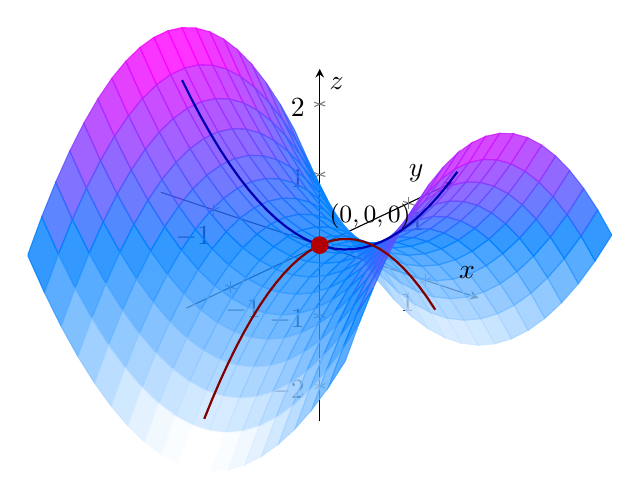
\begin{tikzpicture}
\begin{axis}[
    view={40}{25},
    xlabel={$x$}, ylabel={$y$}, zlabel={$z$},
    axis lines=center,
    tick style={thin},
    zmin=-2.5, zmax=2.5,
    xtick={-1,1}, ytick={-1,1}, ztick={-2,-1,1,2},
    width=9cm, height=9cm,
]
    % Silla de montar: z = x² - y²
    \addplot3[
        surf, shader=flat corner,
        samples=20, domain=-1.5:1.5,
        opacity=0.80, colormap/cool,
    ] {x^2 - y^2};
    % Punto crítico en el origen
    \addplot3[only marks, mark=*, mark size=3pt, red!70!black]
        coordinates {(0,0,0)};
    \node[above right] at (axis cs:0,0,0.1) {\small $(0,0,0)$};
    % Curva de curvatura positiva: y=0, z=x²
    \addplot3[thick, blue!70!black, domain=-1.3:1.3, samples=30, samples y=0]
        ({x},{0},{x^2});
    % Curva de curvatura negativa: x=0, z=-y²
    \addplot3[thick, red!50!black, domain=-1.3:1.3, samples=30, samples y=0]
        ({0},{x},{-x^2});
\end{axis}
\end{tikzpicture}
\caption{Punto de silla en el origen de $z=x^2-y^2$: curvatura positiva
         en dirección $x$ (azul) y negativa en dirección $y$ (rojo)}
\label{fig:punto_silla}
\end{figure}


El siguiente resultado garantiza la existencia de extremos absolutos para
funciones continuas sobre conjuntos cerrados y acotados.

\begin{theorem}[Teorema del Valor Extremo de Weierstrass]
Si $f$ es una función continua de dos variables en un conjunto $S$ que es
\textbf{cerrado} y \textbf{acotado}, entonces $f$ alcanza un valor
máximo absoluto y un valor mínimo absoluto en $S$.
\end{theorem}

\begin{rem}
Las hipótesis de cerradura y acotación son esenciales. Si el conjunto no
es cerrado, el extremo puede ocurrir en la frontera que no pertenece al
dominio. Si no es acotado, la función puede crecer o decrecer
indefinidamente. En una variable, el intervalo $[a,b]$ es el análogo de
un conjunto cerrado y acotado en $\mathbb{R}^2$.
\end{rem}

\begin{pasos}[Localización de extremos absolutos en un conjunto cerrado y acotado]
Para encontrar los extremos absolutos de $f$ en un conjunto $S$ cerrado y
acotado:
\begin{enumerate}
    \item \textbf{Puntos críticos interiores.} Encontrar todos los
    puntos críticos de $f$ en el interior de $S$ (donde $f_x=f_y=0$ o no
    existen).
    \item \textbf{Frontera.} Parametrizar la frontera de $S$ y reducir el
    problema a funciones de una variable sobre cada segmento de la
    frontera. Encontrar los puntos críticos de estas funciones
    unidimensionales, junto con los vértices o esquinas.
    \item \textbf{Evaluación.} Evaluar $f$ en todos los puntos candidatos
    obtenidos en los pasos 1 y 2.
    \item \textbf{Comparación.} El mayor valor es el máximo absoluto; el
    menor, el mínimo absoluto.
\end{enumerate}
\end{pasos}

\begin{rem}
En la práctica, el paso 2 (frontera) es el que requiere más atención,
pues la frontera de una región en $\mathbb{R}^2$ suele estar formada por
curvas (segmentos de recta, arcos de circunferencia, etc.) que deben
parametrizarse adecuadamente. Cada segmento de frontera produce una
función de una variable $f(\mathbf{r}(t))$ cuyo dominio es un intervalo
cerrado, donde se aplica el método de localización de extremos en una
variable.
\end{rem}

%%----------------------------------------------------------
\section{Criterio de la segunda derivada}
%%----------------------------------------------------------

El criterio de la segunda derivada para funciones de dos variables
clasifica los puntos críticos donde $f_x=f_y=0$ utilizando las derivadas
parciales de segundo orden.

\begin{definition}[Discriminante o Hessiano]
Para una función $f$ de dos variables con derivadas parciales de segundo
orden continuas, se define el \textbf{discriminante} (o Hessiano) en un
punto $(a,b)$ como:
\[
D(a,b) = f_{xx}(a,b) f_{yy}(a,b) - \bigl[f_{xy}(a,b)\bigr]^2.
\]
\end{definition}

\begin{theorem}[Criterio de la segunda derivada]
Sea $f$ una función con derivadas parciales de segundo orden continuas en
una vecindad de un punto crítico $(a,b)$ donde $f_x(a,b)=0$ y
$f_y(a,b)=0$. Sea $D = f_{xx}f_{yy} - (f_{xy})^2$ evaluado en $(a,b)$.
Entonces:
\begin{enumerate}[a)]
    \item Si $D > 0$ y $f_{xx}(a,b) > 0$, entonces $f(a,b)$ es un
    \textbf{mínimo local}.
    \item Si $D > 0$ y $f_{xx}(a,b) < 0$, entonces $f(a,b)$ es un
    \textbf{máximo local}.
    \item Si $D < 0$, entonces $(a,b)$ es un \textbf{punto de silla}.
    \item Si $D = 0$, el criterio no permite concluir nada (el punto
    puede ser máximo, mínimo o punto de silla).
\end{enumerate}
\end{theorem}

\begin{rem}
El discriminante puede recordarse como el determinante de la matriz
hessiana:
\[
D = \begin{vmatrix}
f_{xx} & f_{xy} \\
f_{yx} & f_{yy}
\end{vmatrix}
= f_{xx} f_{yy} - (f_{xy})^2.
\]
El caso $D=0$ es el único que requiere un análisis adicional, ya que la
información de segundo orden no es suficiente para clasificar el punto
crítico.
\end{rem}

\begin{rem}[Seguimiento de hipótesis]
El criterio de la segunda derivada exige que las derivadas parciales de
segundo orden sean continuas en una vecindad del punto crítico. Si esta
condición falla, el criterio no es aplicable. Por ejemplo, la función
$f(x,y) = x^2 y^2$ tiene un punto crítico en $(0,0)$ donde $D=0$, y la
continuidad de las derivadas segundas no es el problema (son continuas),
sino que $D=0$ es un caso inconcluso. En cambio, funciones con
discontinuidades en las derivadas segundas pueden presentar
comportamientos atípicos que el criterio no captura.
\end{rem}

\begin{pasos}[Clasificación de puntos críticos mediante el criterio de la segunda derivada]
Para clasificar los puntos críticos de $f$:
\begin{enumerate}
    \item \textbf{Puntos críticos.} Resolver el sistema
    $f_x=0$, $f_y=0$ para obtener todos los puntos críticos.
    \item \textbf{Derivadas segundas.} Calcular $f_{xx}$, $f_{xy}$,
    $f_{yy}$.
    \item \textbf{Discriminante.} Para cada punto crítico $(a,b)$,
    calcular $D = f_{xx} f_{yy} - (f_{xy})^2$.
    \item \textbf{Clasificación.} Aplicar el criterio de la segunda
    derivada:
    \begin{itemize}
        \item $D>0$ y $f_{xx}>0$: mínimo local.
        \item $D>0$ y $f_{xx}<0$: máximo local.
        \item $D<0$: punto de silla.
        \item $D=0$: criterio inconcluso.
    \end{itemize}
\end{enumerate}
\end{pasos}

\begin{example}[Clasificación de puntos críticos con punto de silla]
Determine los valores máximos y mínimos locales y los puntos de silla de
$f(x,y) = x^4 + y^4 - 4xy + 1$.
\begin{myproof}
Se sigue el protocolo de clasificación de puntos críticos.

\textbf{Paso 1. Puntos críticos.}
\[
f_x = 4x^3 - 4y = 0 \implies y = x^3.
\]
\[
f_y = 4y^3 - 4x = 0 \implies x = y^3.
\]
Sustituyendo $y=x^3$ en $x=y^3$:
\[
x = (x^3)^3 = x^9 \implies x^9 - x = 0 \implies x(x^8 - 1)=0.
\]
Las raíces reales son $x=0$, $x=1$, $x=-1$. Por tanto, los puntos
críticos son:
\[
(0,0),\qquad (1,1),\qquad (-1,-1).
\]

\textbf{Paso 2. Derivadas segundas.}
\[
f_{xx} = 12x^2,\qquad f_{xy} = -4,\qquad f_{yy} = 12y^2.
\]

\textbf{Paso 3. Discriminante.}
\[
D(x,y) = f_{xx} f_{yy} - (f_{xy})^2
= (12x^2)(12y^2) - (-4)^2
= 144x^2 y^2 - 16.
\]

\textbf{Paso 4. Clasificación.}

\textbf{En $(0,0)$:}
\[
D(0,0) = 0 - 16 = -16 < 0.
\]
Por el caso c) del criterio, $(0,0)$ es un \textbf{punto de silla}.
El valor en el punto es $f(0,0)=1$.

\textbf{En $(1,1)$:}
\[
D(1,1) = 144(1)(1) - 16 = 128 > 0,
\]
\[
f_{xx}(1,1) = 12 > 0.
\]
Por el caso a), $f(1,1) = 1 + 1 - 4 + 1 = -1$ es un
\textbf{mínimo local}.

\textbf{En $(-1,-1)$:}
\[
D(-1,-1) = 144(1)(1) - 16 = 128 > 0,
\]
\[
f_{xx}(-1,-1) = 12 > 0.
\]
Por el caso a), $f(-1,-1) = 1 + 1 - 4 + 1 = -1$ es un
\textbf{mínimo local}.

Por tanto:
\[
\boxed{
\text{Punto de silla: } (0,0,1),\quad
\text{Mínimos locales: } (1,1,-1),\ (-1,-1,-1)
}.
\]
\end{myproof}
\end{example}

\begin{rem}
El ejemplo muestra un fenómeno que no ocurre en funciones de una
variable: el punto de silla. En $(0,0)$, la función crece en las
direcciones de los ejes (pues $x^4$ y $y^4$ son positivos) pero decrece
en las direcciones diagonales (pues el término $-4xy$ domina cerca del
origen). Esta geometría se asemeja a una silla de montar: el punto
central es un mínimo en una dirección y un máximo en otra, sin ser ni uno
ni otro.
\end{rem}

%%==========================================================
\begin{prob}
Determine el punto sobre el plano $x-y+z=9$ que está más cerca al punto $(1,2,5).$
\begin{myproof}
La función de distancia es $s=(x-1)^2+(y-2)^2+(z-5)^2$ (recuerde que minimizar $s$ minimiza su cuadrado) pero se está calculando la distancia a un punto que pertenece al plano $x-y+z-9=0.$ Despejando a $z$ de la ecuación del plano se obtiene la función $s=(x-1)^2+(y-2)^2+(4-x+y)^2$ la cual se va a minimizar.
Calculando las derivadas, $$\dfrac{\partial s}{\partial x}=2(x-1)-2(4-x+y)$$ y  $$\dfrac{\partial s}{\partial y}=2(y-2)+2(4-x+y).$$
\begin{multicols}{2}
Haciendo $\dfrac{\partial s}{\partial x}=0$ se obtiene:
\begin{align*}
0&=2x-2-8+2x-2y\\
0&=4x-2y-10.
\end{align*}
\columnbreak
Similarmente, si $\dfrac{\partial s}{\partial y}=0$ entonces:
\begin{align*}
0&=2y-4+8-2x+2y\\
0&=4y-2x+4.
\end{align*}
\end{multicols}
Lo cual lleva a resolver el siguiente sistema de ecuaciones
\begin{align*}
0&=4x-2y-10\\0&=4y-2x+4
\end{align*}
Cuya solución es $x=\dfrac{8}{3}$ y $y=\dfrac{1}{3}.$
Por criterio de las segundas derivadas parciales, al calcular 
\begin{multicols}{3}
$$\dfrac{\partial^2 s}{\partial x^2}=4,$$ $$\dfrac{\partial^2 s}{\partial y^2}=4,$$ $$\dfrac{\partial^2 s}{\partial x\partial y}=-2.$$
\end{multicols}
Evaluando el valor de $D$ en el punto $\left( \dfrac{8}{3},\dfrac{1}{3}  \right)$:
$D=\left(\dfrac{\partial^2 s}{\partial x^2}\right)\left(\dfrac{\partial^2 s}{\partial y^2}\right)-\left(\dfrac{\partial^2 s}{\partial x\partial y}\right)^2=\left(  4  \right)\left( 4 \right)-\left(-2 \right)^2 = 12>0$
Finalmente,  $$\dfrac{\partial^2 s}{\partial x^2}=4>0$$
Lo cual implica que $\left( \dfrac{8}{3},\dfrac{1}{3}  \right)$ es un mínimo. Así el punto más cercano es $\left(\dfrac{8}{3},\dfrac{1}{3},\dfrac{20}{3}\right)$
La distancia mínima será $s=\sqrt{\left(\dfrac{8}{3}-1\right)^2+\left(\dfrac{1}{3}-2\right)^2+\left(4-\dfrac{8}{3}+\dfrac{1}{3}\right)^2}=\dfrac{5\sqrt{3}}{3}.$
\end{myproof}
\end{prob}

\begin{prob}
Se construirá un canal abierto con sección transversal en la forma de un  trapecio con ángulos iguales en la base, doblando franjas iguales a ambos lados de una larga pieza de metal de 50 centímetros de ancho tal como se muestra en la figura. Determine los ángulos en la base y el ancho de los lados para obtener la mayor capacidad de carga.
\begin{myproof}
\begin{figure}[H]
\centering
\begin{tikzpicture}[line cap=round,line join=round,>=triangle 45,x=1.0cm,y=1.0cm]
\clip(-0.9631690910028438,-1.0185175531939794) rectangle (9.64234461356722,3.9917251304360035);
\draw [shift={(6.,0.)},line width=2.pt] (0,0) -- (0.:0.4500217979308372) arc (0.:56.309932474020215:0.4500217979308372) -- cycle;
\draw [shift={(2.,0.)},line width=2.pt] (0,0) -- (123.6900675259798:0.4500217979308372) arc (123.6900675259798:180.:0.4500217979308372) -- cycle;
\draw [shift={(8.,3.)},line width=2.pt] (0,0) -- (180.:0.4500217979308372) arc (180.:236.3099324740202:0.4500217979308372) -- cycle;
\draw [shift={(0.,3.)},line width=2.pt,] (0,0) -- (-56.309932474020215:0.4500217979308372) arc (-56.309932474020215:0.:0.4500217979308372) -- cycle;
\draw [line width=5.2pt] (0.,3.)-- (2.,0.);
\draw [line width=5.2pt] (2.,0.)-- (6.,0.);
\draw [line width=5.2pt] (6.,0.)-- (8.,3.);
\draw [line width=5.2pt] (8.,3.)-- (0.,3.);
\draw [line width=2.pt] (2.,0.)-- (2.,3.);
\draw [line width=2.pt] (6.,0.)-- (6.,3.);
\draw (0.46189993577814065,1.5616074216094848) node[anchor=north west] {$x$};
\draw (6.522193481246748,3.676709871884418) node[anchor=north west] {$x\cos \theta$};
\draw (0.5969064751573918,3.7967156846659744) node[anchor=north west] {$x\cos \theta$};
\draw (3.3420394425354987,-0.0734717775392221) node[anchor=north west] {$50-2x$};
\draw (2.1419813147199327,1.936625586551849) node[anchor=north west] {$x \sin \theta$};
\draw (4.5,1.9216248599541543) node[anchor=north west] {$x \sin \theta$};
\draw (7.242228357936088,1.5766081482071794) node[anchor=north west] {$x$};
\draw [line width=2.pt,domain=-0.9631690910028438:9.64234461356722] plot(\x,{(-0.-0.*\x)/6.});
\draw[color=black] (6.8,0.38405038369046196) node {$\theta $};
\draw[color=black] (1.3019406252490366,0.39905111028815654) node {$\theta $};
\draw[color=black] (7.1,2.6) node {$\theta $};
\draw[color=black] (0.7,2.6) node {$\theta$};
\end{tikzpicture}
 \end{figure}
Para hallar el canal con volumen máximo basta con maximizar el área de la sección transversal, formado por el trapecio de la figura. Como el área de un trapecio está dada por la fórmula $A=\dfrac{B+b}{2}h$ donde $B$ es la base mayor, $b$ la base menor y $h$ la altura, se debe maximizar la función $A(x,\theta)=\dfrac{B+b}{2}h,$ donde $x$ es la longitud del canal que se dobla y $\theta$ es el ángulo desde la base del canal.
Por la figura puede observarse que:
\begin{multicols}{3}
\begin{itemize}
\item $B=2x\cos \theta + 50-2x.$
\item $b=50-2x.$
\item $h=x\sin \theta.$
\end{itemize}
\end{multicols}
Lo cual implica que la función de área queda determinada por
\begin{align*}
A(x,\theta)&=\dfrac{1}{2}\left[ 2x\cos \theta+(50-2x)+(50-2x) \right]x\sin \theta,\\
&=\left(x\cos \theta+(50-2x)\right)x\sin \theta,\\
&=x^2\cos\theta \sin \theta+50x\sin \theta-2x^2\sin \theta.
\end{align*}
Como los puntos críticos de la función están donde las dos primeras derivadas parciales son cero, se hace el cálculo de estas derivadas y  después se encuentran los puntos donde son simultáneamente cero. Así,
\begin{itemize}
\item $\dfrac{\partial A}{\partial x}=2x\cos\theta\sin\theta +50\sin \theta -4x\sin \theta.$
\item $\dfrac{\partial A}{\partial \theta}=50 x \cos \theta -2 x^2\cos \theta +x^2\left(cos^{2}\theta-\sin^{2}\theta\right)=50 x \cos \theta -2 x^2\cos \theta +x^2\left(2cos^{2}\theta-1\right).$  
\end{itemize}
Si $\dfrac{\partial A}{\partial x}=0$ entonces $\sin \theta \left( 2x\cos\theta +50-4x \right)=0.$ Como $\sin \theta=0$ si $\theta =0$ o $\theta =\pi$ se descartan esos puntos, por lo cual se tomará el caso cuando $2x\cos\theta +50-4x =0,$ lo cual implica que $\cos \theta=\dfrac{2x-25}{x}.$
Como las primeras derivadas parciales deben ser cero simultáneamente, puede hacerse el reemplazo $\cos \theta=\dfrac{2x-25}{x}$ en la ecuación $\dfrac{\partial A}{\partial \theta}=0.$ 
De esta manera, haciendo los cálculos correspondientes se obtiene que
\begin{align*}
0=\dfrac{\partial A}{\partial \theta}&=50x\left(\dfrac{2x-25}{x}\right)-2x^2\left(\dfrac{2x-25}{x}\right)+x^2\left(2\left(\dfrac{2x-25}{x}\right)^{2}-1\right),\\
0&=50\left(2x-25\right)-2x\left(2x-25\right)+2\left( 2x-25 \right)^2-x^2,\\
0&=3x^2-50x,\\
0&=x(3x-50).\\
\end{align*}
Así, $x=0$  o $x=\dfrac{50}{3},$ como $x>0$ se toma el punto $x=\dfrac{50}{3},$ y esto determina que $\cos \theta =\dfrac{-2+2\left( \frac{50}{3} \right)}{\frac{50}{3}}=\dfrac{1}{2}$  y así $\theta=\frac{\pi}{3}.$ 
Finalmente, el punto para el cual el volumen del canal es máximo son los puntos $(x,\theta)=\left(\dfrac{50}{3},\dfrac{\pi}{3}\right).$ 
\end{myproof}
\end{prob}

\begin{prob}
El material para construir la base de una caja cuya tapa es abierta cuesta $1.5$ veces más por unidad de área que el material para los lados. Si hay disponibles $\$ 1 000$, halle la caja de mayor volumen que puede ser fabricada.
\begin{myproof}
Sea $x,\ y,\ z$ la longitud de costo del ancho, el largo y la altura de la caja respectivamente. Note que el área superficial de la caja es $A_{s}=2xz+2yz+xy$ y el costo de su producción está dado por la función $C(x,y)=2xz+2yz+1.5xy.$ Como el valor destinado para su producción es $\$ 1000$, se tiene que, $1000=C(x,y)=2xz+2yz+1.5xy,$ donde se puede despejar $z$ obteniendo $z=\dfrac{1000-1.5xy}{2x+2y}.$  
Así, el volumen de la caja está dado por $$V= xy   \left(\dfrac{1000-1.5xy}{2x+2y}\right)=\dfrac{1000xy-1.5x^2y^2}{2x+2y}.$$
Al calcular las primeras derivadas parciales se tiene que
\begin{itemize}
\item $\dfrac{\partial V}{\partial x}=\dfrac{\left( 1000y-3xy^2 \right)\left( 2x+2y \right)-2\left( 1000xy-1.5x^2y^2 \right)}{\left(2x+2y\right)^{2}}=\dfrac{y^{2}\left(2000-3x^2-6xy\right)}{4\left(x+y\right)^{2}}.$
\item $\dfrac{\partial V}{\partial y}=\dfrac{\left( 1000x-3x^2y \right)\left( 2x+2y \right)-2\left( 1000xy-1.5x^2y^2 \right)}{\left(2x+2y\right)^{2}}=\dfrac{x^{2}\left(2000-3y^2-6xy\right)}{4\left(x+y\right)^{2}}.$
\end{itemize}
Observe que las dos primeras derivadas parciales son iguales si $y=x,$ por lo tanto basta hacer este cambio en una de ellas para obtener los puntos críticos. 
En efecto, $0=\dfrac{x^2\left( 2000-3x^2-6x^2 \right)}{4\left( 2x \right)^2}=\dfrac{x^2\left( 2000-9x^2 \right)}{16x^2}.$ 
Es decir, $0=x^2\left( 2000-9x^2 \right).$ De ahí, $x=0,$ $x=\pm \sqrt{\dfrac{2000}{9}}=\pm \dfrac{20\sqrt{5}}{3},$ que determina el único valor $x=\dfrac{20\sqrt{5}}{3},$ el cual es un máximo (puede comprobarlo con el criterio de la segunda derivada), que determina las dimensiones de la caja como $x=\dfrac{20\sqrt{5}}{3},$ $y=\dfrac{20\sqrt{5}}{3},$ $z=5\sqrt{5}.$ 
Finalmente, el volumen es aproximadamente $V=\left( \dfrac{20\sqrt{5}}{3} \right)\left( \dfrac{20\sqrt{5}}{3} \right)\left( 5\sqrt{5} \right)\approx 2484.52$ unidades cúbicas.
\end{myproof}
\end{prob}

\begin{prob}
Calcule el volumen de la caja rectangular más grande en el primer octante con tres caras en los planos coordenados y un vértice en el plano $x+5y+3z=6.$
\begin{myproof}
Como la caja está en el primer cuadrante, el volumen es $V=xyz,$ pero se conoce que un vértice de esta se encuentra sobre el plano $x+5y+3z=6.$ Despejando a $z$ de la ecuación del plano se obtiene la función $V=\dfrac{xy}{3}\left( 6-x-5y \right)$ la cual se va a maximizar.
Calculando las derivadas, $$\dfrac{\partial V}{\partial x}=2y-\frac{2}{3}xy-\frac{5}{3}y^2$$ y  $$\dfrac{\partial V}{\partial y}=2x-\frac{10}{3}xy-\frac{1}{3}x^2.$$
\begin{multicols}{2}
Haciendo $\dfrac{\partial V}{\partial x}=0$ se obtiene:
\begin{align*}
0&=2y-\frac{2}{3}xy-\frac{5}{3}y^2\\
&=y\left(2-\frac{2}{3}x-\frac{5}{3}y\right)\\
&\Rightarrow y=0 \text{ o } y=\dfrac{6-2x}{5}.
\end{align*}
\columnbreak
Similarmente, si $\dfrac{\partial V}{\partial y}=0$ entonces:
\begin{align*}
0&=2x-\frac{10}{3}xy-\frac{1}{3}x^2\\
&=x\left(2-\frac{1}{3}x-\frac{10}{3}y\right)\\
&\Rightarrow x=0 \text{ o } y=\dfrac{6-x}{10}.
\end{align*}
\end{multicols}
Lo cual da dos puntos críticos: $(0,0)$ y el que resulta de igualar los valores de $y.$
Así, 
\begin{align*}
\dfrac{6-2x}{5}&=\dfrac{6-x}{10}\\\dfrac{6}{5}-\dfrac{3}{5}&=\dfrac{4x}{10}-\dfrac{x}{10}\\\dfrac{3}{5}&=\dfrac{3x}{15}\\30&=15x\\x&=2.
\end{align*}
Como $x=2,$ entonces $y=\dfrac{2}{5}.$  
Por criterio de las segundas derivadas parciales, al calcular 
\begin{multicols}{3}
$$\dfrac{\partial^2 V}{\partial x^2}=\dfrac{-2}{3}y,$$ $$\dfrac{\partial^2 V}{\partial y^2}=\dfrac{-10}{3}x,$$ $$\dfrac{\partial^2 V}{\partial x\partial y}=2-\dfrac{2x}{3}-\dfrac{10y}{3}.$$
\end{multicols}
Evaluando el valor de $D$ en el punto $\left( 2,\dfrac{2}{5}  \right)$:
$D=\left(\dfrac{\partial^2 V}{\partial x^2}\right)\left(\dfrac{\partial^2 V}{\partial y^2}\right)-\left(\dfrac{\partial^2 V}{\partial x\partial y}\right)^2=\left(  \dfrac{-4}{15}  \right)\left(  \dfrac{-20}{3}  \right)-\left( -\dfrac{2}{3} \right)^2 = \dfrac{4}{3}>0$
Finalmente,  $$\dfrac{\partial^2 V}{\partial x^2}=\dfrac{-2}{3}y=\dfrac{-4}{15}<0$$
Lo cual implica que $\left( 2,\dfrac{2}{5}  \right)$ es un máximo.
El volumen de la caja será $V=\dfrac{xy}{3}\left( 6-x-5y \right)=\dfrac{8}{15}\ u^3.$
\end{myproof}
\end{prob}

\begin{prob}
La base de un acuario de volumen $V$ está hecho de cerámica y los lados son de vidrio. Si la cerámica cuesta tres veces más por unidad de área que el vidrio, determine las dimensiones del acuario que minimizan el costo de los materiales.
\begin{myproof}
Sean $x,$ $y$ y $z$ las dimensiones del ancho, el largo y la altura del acuario. Por lo tanto, el área de la cerámica será $xy.$ Sea $V=xyz$ el volumen del acuario, entonces $z=\dfrac{V}{xy}$ y como el área superficial del acuario es $A=2(xz+yz)+xy$ la función de costo es $C=3xy+2xz+2yz$ la cual se convierte al reemplazar $z$ en $C=3xy+\dfrac{2V}{y}+\dfrac{2V}{x}.$ 
Calculando las derivadas, $$\dfrac{\partial C}{\partial x}=3y-\dfrac{2V}{x^2}$$ y  $$\dfrac{\partial C}{\partial y}=3x-\dfrac{2V}{y^2}.$$
\begin{multicols}{2}
Haciendo $\dfrac{\partial C}{\partial x}=0$ se obtiene:
\begin{align*}
0&=3y-\dfrac{2V}{x^2}\\
y&=\dfrac{2V}{3x^2}.
\end{align*}
\columnbreak
Similarmente, si $\dfrac{\partial C}{\partial y}=0$ entonces:
\begin{align*}
0&=3x-\dfrac{2V}{y^2}\\
x&=\dfrac{2V}{3y^2}.
\end{align*}
\end{multicols}
Resolviendo,
$$3x=\dfrac{2V}{y^2}\Leftrightarrow 3x=\dfrac{2V}{\left( \dfrac{2V}{3x^2} \right)^2} \Leftrightarrow 3x=\dfrac{2V(9x^4)}{4V^2}\Leftrightarrow x^3=\dfrac{2V}{3}\Leftrightarrow x=\sqrt[3]{\dfrac{2V}{3}}.$$
Observando la otra ecuación, $y=\sqrt[3]{\dfrac{2V}{3}}.$
 
Por criterio de las segundas derivadas parciales, al calcular 
\begin{multicols}{3}
$$\dfrac{\partial^2 C}{\partial x^2}=\dfrac{4V}{x^3},$$ $$\dfrac{\partial^2 C}{\partial y^2}=\dfrac{4V}{y^3},$$ $$\dfrac{\partial^2 C}{\partial x\partial y}=3.$$
\end{multicols}
Evaluando el valor de $D$ en el punto $\left( \sqrt[3]{\dfrac{2V}{3}},\sqrt[3]{\dfrac{2V}{3}} \right)$:
$D=\left(\dfrac{\partial^2 s}{\partial x^2}\right)\left(\dfrac{\partial^2 s}{\partial y^2}\right)-\left(\dfrac{\partial^2 s}{\partial x\partial y}\right)^2=\left(  6  \right)\left( 6 \right)-\left(3 \right)^2 = 27>0$
Finalmente,  $$\dfrac{\partial^2 s}{\partial x^2}=6>0$$
Lo cual implica que $\left( \sqrt[3]{\dfrac{2V}{3}},\sqrt[3]{\dfrac{2V}{3}} \right)$ es un mínimo. Así las dimensiones son $\left( \sqrt[3]{\dfrac{2V}{3}},\sqrt[3]{\dfrac{2V}{3}},\left(\dfrac{3}{2}\right)^{2/3}\sqrt[3]{V} \right)=\left( \sqrt[3]{\dfrac{2V}{3}},\sqrt[3]{\dfrac{2V}{3}},\sqrt[3]{\left(\dfrac{9}{4}\right){V}} \right).$
\end{myproof}
\end{prob}

\begin{prob}
\textbf{Ley de Hardy-Weinberg} Los tipos sanguíneos son genéticamente determinados por tres alelos A, B y O. (Alelo es cualquiera de las posibles formas de mutación de un gen.) Una persona cuyo tipo sanguíneo es AA, BB u OO es homocigótica. Una persona cuyo tipo sanguíneo es AB, AO o BO es heterocigótica. La ley Hardy-Weinberg establece que la proporción $P$ de individuos heterocigótica en cualquier población dada es $P(p,q,r)=2pq+2pr+2qr,$  donde $p$ representa el porcentaje de alelos A en la población, $q$ representa el porcentaje de alelos B en la población y $r$ representa el porcentaje de alelos O en la población. Utilizar el hecho que $p+q+r=1$ para mostrar que la proporción máxima de individuos heterocigóticos en cualquier población es $\dfrac{2}{3}.$
\begin{myproof}
Sea $P(p,q,r)=2pq+2pr+2qr$ la proporción de individuos heterocigóticos. Como $p=1-q-r$ la función de proporción se reduce a $P(q,r)=2(1-q-r)q+2(1-q-r)r+2qr=-2q^2-2r^2-2qr+2q+2r.$ 
Al calcular las primeras derivadas parciales,
\begin{itemize}
\item $\dfrac{\partial P}{\partial r}=-4r-2q+2.$
\item $\dfrac{\partial P}{\partial q}=-4q-2r+2.$
\end{itemize}
Note que $\dfrac{\partial P}{\partial r}=-4r-2q+2=0$ implica que $4r+2q=2$ y de manera análoga $\dfrac{\partial P}{\partial q}=-4q-2r+2=0$ implica que $2r+4q=2.$
La solución del sistema de ecuaciones $\left\lbrace \begin{array}{ccc} 2&=&4r+2q\\
2&=&2r+4q \end{array} \right.$ determina a $\left(\dfrac{1}{3},\dfrac{1}{3}\right)$ como punto crítico.
Al usar el criterio de las segundas derivadas parciales, como $P_{rr}=-4,\ P_{qq}=-4$ y $P_{qr}=-2,$ $D=\left(-4\right)\left(-4\right)-\left( -2 \right)^{2}=12>0.$ Lo cual dice que $\left( \dfrac{1}{3},\dfrac{1}{3} \right)$ es un máximo.
Finalmente, al despejar,  $p= \dfrac{1}{3}.$ Esto lleva a que la proporción  $P\left(\dfrac{1}{3},\dfrac{1}{3},\dfrac{1}{3}  \right)=\dfrac{2}{3}$ tal como se quería demostrar.
\end{myproof}
\end{prob}

\begin{prob}
Determine el punto en el plano $2x+4y+3z=12$ que es más cercano al origen.
\begin{myproof}
Sea $P(x,y,z)$ un punto en el plano. Entonces el cuadrado de la distancia entre el origen y $P$ es $d^2=x^2+y^2+z^2.$ Como $P$ está en el plano, $z=\dfrac{12-2x-4y}{3},$ por lo cual se quiere minimizar  $d^2=f(x,y)=x^2+y^2+\left( \dfrac{12-2x-4y}{3} \right)^{2}.$
Al calcular las derivadas parciales se obtiene que 
\begin{itemize}
\item $\dfrac{\partial f}{\partial x}=2x+\dfrac{2}{9}\left( 12-2x-4y \right)(-2)=\dfrac{-48+26x+16y}{9}.$
\item $\dfrac{\partial f}{\partial y}=2y+\dfrac{2}{9}\left( 12-2x-4y \right)(-4)=\dfrac{-96+16x+50y}{9}.$
\end{itemize}
Así, $\dfrac{\partial f}{\partial x}=0=\dfrac{-48+26x+16y}{9}$ implica que $24=13x+8y.$ 
Análogamente, $\dfrac{\partial f}{\partial y}=0=\dfrac{-96+16x+50y}{9}$ implica que $48=8x+25y.$ 
Al resolver el sistema de ecuaciones $\left\lbrace \begin{array}{ccc} 24&=&13x+8y\\
48&=&8x+25y \end{array} \right.$ se obtiene el punto crítico $\left( \dfrac{24}{29},\dfrac{48}{29} \right).$ 
Al usar el criterio de las segundas derivadas parciales, como $f_{xx}=\dfrac{26}{9},\ f_{yy}=\dfrac{50}{9}$ y $f_{xy}=\dfrac{16}{9},$ $D=\left(\dfrac{26}{9}\right)\left(\dfrac{50}{9}\right)-\left( \dfrac{16}{9} \right)^{2}=\dfrac{116}{9}>0.$ Lo cual dice que $\left( \dfrac{24}{29},\dfrac{48}{29} \right)$ es un mínimo.
Finalmente, al despejar,  $z=\dfrac{12-2\left( \frac{24}{29} \right)-4\left( \frac{48}{29} \right)}{3}=\dfrac{36}{29}, $ por lo cual el punto  cuya distancia es mínima es $\left(\dfrac{24}{29},\dfrac{48}{29},\dfrac{36}{29}  \right).$ 
\end{myproof}
\end{prob}
\begin{prob}
Suponga que la temperatura $T$ en la placa circular $\{  (x,y): x^2+y^2\leq 1 \}$ está dada por la función $T(x,y)=2x^2+y^2-y.$ Determine cuáles son los puntos más calientes y más fríos de la placa.
\begin{myproof} 
Para observar donde ocurre este fenómeno se calculan inicialmente los puntos críticos  donde las primeras derivadas parciales son cero. 
Así, $\dfrac{\partial T}{\partial x}=4x$ y $\dfrac{\partial T}{\partial y}=2y-1,$ las cuales se anulan en el punto $(0,\frac{1}{2}),$ y este es el primer punto crítico. 
Como los puntos de frontera  de la placa también son críticos, hay que verificar si son máximos o mínimos. La frontera está determinada por la ecuación $x^2+y^2=1$ entonces $x^2=1-y^2,$ y así $T(y)=2(1-y^2)+y^2-y=-y^2-y+2.$ Esta función tiene dominio $\left[-1,1\right],$ por lo cual dos de los puntos a evaluar como máximo o mínimo son $(0,-1)$ y $(0,1).$
Observe que $T^{\prime}(y)=-2y-1,$ se obtienen sus puntos críticos haciendo  $T^{\prime}(y)=0,$ obteniendo el punto $y=\dfrac{-1}{2},$ y así otros posibles candidatos son los puntos $\left( \dfrac{\sqrt{3}}{2}, \dfrac{-1}{2} \right)$ y $\left( \dfrac{-\sqrt{3}}{2}, \dfrac{1}{-2} \right).$ 
 
 Finalmente se evalúan todos los puntos para verificar cuál es máximo o mínimo.
 \begin{multicols}{3}
 \begin{itemize}
 \item $T\left(0,\dfrac{1}{2}\right)=\dfrac{-1}{4}.$
 \item $T\left(0,-1\right)=2.$
 \item $T\left(0,1\right)=0.$
 \item $T\left(\dfrac{\sqrt{3}}{2},-\dfrac{1}{2}\right)=\dfrac{9}{4}.$
  \item $T\left(-\dfrac{\sqrt{3}}{2},-\dfrac{1}{2}\right)=\dfrac{9}{4}.$
 \end{itemize}
\end{multicols}
De donde se puede concluir que los puntos donde la temperatura es más alta son $\left( \dfrac{\sqrt{3}}{2}, \dfrac{-1}{2} \right)$ y $\left( \dfrac{-\sqrt{3}}{2}, \dfrac{1}{-2} \right).$ El punto donde la temperatura es más baja es  $\left(0,\dfrac{1}{2}\right).$
\end{myproof}
\end{prob}
\section{Optimización restringida y multiplicadores de Lagrange}

Estudiaremos la optimización de funciones restringidas usando un ejemplo motivador

\begin{prob}[Rectángulo de diagonal fija]
Determine el área máxima de un rectángulo cuya diagonal mide $d>0$.
\end{prob}

Colocamos un vértice en el origen y el opuesto en $(x,y)$ con $x,y>0$; la diagonal satisface $\sqrt{x^2+y^2}=d$. El problema es

\[
\text{Maximizar } f(x,y)=xy \quad \text{sujeta a } g(x,y)=x^2+y^2-d^2=0,\quad x,y>0.
\]

La pregunta que guía el desarrollo es: ¿cómo hallar el máximo \emph{sin} eliminar una variable? La respuesta la proporciona el método de Lagrange, que se apoya en la relación geométrica entre las curvas de nivel de $f$ y la restricción.



Note que, para la función objetivo a minimizar en el problema del rectángulo las curvas de nivel de $f(x,y)=xy$ son hipérbolas $xy=C$, y la restricción $g=0$ es una circunferencia. Si en un punto de la circunferencia se alcanza el máximo de $f$ restringido, la hipérbola que pasa por ese punto debe ser \textbf{tangente} a la circunferencia; de otro modo, moviéndonos ligeramente sobre la circunferencia podríamos aumentar el área. Para justificar esta tangencia necesitamos el concepto de curva regular y el teorema de la función implícita.

\begin{definition}[Curva regular]
Una \textbf{curva regular} en $\R^2$ es una función diferenciable $\mathbf{r}\colon I\subset\R\to\R^2$, $\mathbf{r}(t)=(x(t),y(t))$, tal que $\mathbf{r}'(t)\neq\mathbf{0}$ para todo $t\in I$.
\end{definition}

\begin{theorem}[Función implícita]
Si $g\colon\R^2\to\R$ es de clase $\mathcal C^1$ y $\nabla g(x_0,y_0)\neq\mathbf{0}$ con $g(x_0,y_0)=0$, entonces en un abierto de $(x_0,y_0)$ la ecuación $g(x,y)=0$ define una curva regular (localmente expresable como $y=\varphi(x)$ o $x=\psi(y)$).
\end{theorem}

En el problema del rectángulo, $\nabla g=(2x,2y)$ se anula únicamente en el origen, que no pertenece a la restricción ($d>0$); por tanto, todos los puntos de la circunferencia son regulares y el teorema de la función implícita garantiza que la restricción es localmente una curva suave.

\begin{prop}[Ortogonalidad del gradiente a las curvas de nivel]
Sea $f$ diferenciable y sea $\mathbf{r}(t)$ una curva regular contenida en la curva de nivel $f(\mathbf{r}(t))=c$. Entonces $\nabla f(\mathbf{r}(t))$ es perpendicular a $\mathbf{r}'(t)$ para cada $t$.
\end{prop}

\begin{proof}
Derivando $f(\mathbf{r}(t))=c$ respecto a $t$ mediante la regla de la cadena:
\[
\nabla f(\mathbf{r}(t))\cdot \mathbf{r}'(t)=0.
\]
El producto escalar nulo caracteriza la ortogonalidad.
\end{proof}

En particular, para la restricción $g=0$, el vector $\nabla g$ es perpendicular a la curva $\{g=0\}$ en cada punto regular.

Si parametrizamos la restricción $g=0$ mediante una curva regular $\mathbf{r}(t)$ y definamos $h(t)=f(\mathbf{r}(t))$. Si en $t_0$ la función $h$ alcanza un extremo local (porque $\mathbf{r}(t_0)$ es extremo de $f$ sobre la restricción), entonces $h'(t_0)=0$, es decir,
\[
\nabla f(\mathbf{r}(t_0))\cdot \mathbf{r}'(t_0)=0.
\]
Así, $\nabla f$ es perpendicular al vector tangente $\mathbf{r}'(t_0)$. Por la proposición anterior, $\nabla g$ también es perpendicular a $\mathbf{r}'(t_0)$. En $\R^2$, dos vectores perpendiculares a una misma recta son paralelos; por tanto, existe $\lambda\in\R$ tal que
\[
\nabla f(\mathbf{r}(t_0)) = \lambda\,\nabla g(\mathbf{r}(t_0)).
\]
Este escalar $\lambda$ se denomina \textbf{multiplicador de Lagrange}. La igualdad vectorial equivale a un sistema de $n$ ecuaciones (más la restricción) en $n+1$ incógnitas.

\section{Teorema de los Multiplicadores de Lagrange}

\begin{theorem}[Multiplicadores de Lagrange, condición necesaria]
Sean $f$ y $g$ funciones de clase $\mathcal C^1$ en un abierto de $\R^n$. Si $\mathbf{x}_0$ es un extremo local de $f$ restringido a la superficie $g(\mathbf{x})=0$ y $\nabla g(\mathbf{x}_0)\neq \mathbf{0}$, entonces existe un escalar $\lambda$ tal que
\[
\nabla f(\mathbf{x}_0) = \lambda\,\nabla g(\mathbf{x}_0).
\]
Equivalentemente, definiendo la \textbf{función de Lagrange}
\[
F(\mathbf{x},\lambda)=f(\mathbf{x})+\lambda g(\mathbf{x}),
\]
la condición anterior junto con $g(\mathbf{x}_0)=0$ equivale a $\nabla F(\mathbf{x}_0,\lambda)=\mathbf{0}$.
\end{theorem}

\begin{rem}
El teorema establece una condición \emph{necesaria, no suficiente}: los puntos que satisfacen $\nabla F=\mathbf{0}$ son solo candidatos a extremo. Se requiere un análisis adicional para determinar su naturaleza.
\end{rem}

El siguiente teorema garantiza la existencia de extremos cuando la restricción es compacta.

\begin{theorem}[Weierstrass]
Sea $K\subset\R^n$ compacto (cerrado y acotado) y $f\colon K\to\R$ continua. Entonces $f$ alcanza su máximo y su mínimo absolutos en $K$.
\end{theorem}

Si la restricción $S$ es compacta, el teorema de Weierstrass asegura la existencia de extremos absolutos; si además la regularidad se cumple en todos los puntos de $S$, todo extremo aparece como candidato de Lagrange, por lo que basta evaluar $f$ en todos los candidatos y comparar.

\begin{figure}[H]
\centering
\begin{tikzpicture}[scale=1.2]
    \draw[thin,->] (-2.3,0) -- (2.5,0) node[right] {$x$};
    \draw[thin,->] (0,-2.3) -- (0,2.5) node[above] {$y$};
    % Curvas de nivel f(x,y)=x²+y²/2 para c=0.5,1,1.5,2 (elipses)
    % Semiejes: a=√c, b=√(2c)
    \foreach \c/\col in {0.5/blue!20!black, 1/blue!40!black, 1.5/blue!60!black, 2/blue!80!black}{
        \pgfmathsetmacro{\a}{sqrt(\c)}
        \pgfmathsetmacro{\b}{sqrt(2*\c)}
        \draw[thick, \col] (0,0) ellipse ({\a} and {\b});
    }
    % Restricción g(x,y)=x+y-1=0 (recta x+y=1)
    \draw[thick, red!70!black, domain=-1.4:2.4, variable=\t, samples=2]
        plot ({\t},{1-\t});
    \node[anchor=south west, red!70!black] at (1.8,-0.8)
        {\small $g=x+y-1=0$};
    % Punto de tangencia: mínimo de f sobre la recta
    % f restringida: f(t,1-t)=t²+(1-t)²/2; f'=2t-(1-t)=3t-1=0 → t=1/3
    % Punto: (1/3, 2/3)
    \filldraw[red!70!black] ({1/3},{2/3}) circle (2pt)
        node[anchor=south west] {\small $({\tfrac{1}{3}},{\tfrac{2}{3}})$};
    % Gradiente de f en el punto: ∇f=(2/3, 2/3)·0.35 → (0.233, 0.233)
    \draw[->, thick, green!50!black]
        ({1/3},{2/3}) -- ({1/3+0.233},{2/3+0.233});
    \node[anchor=west, green!50!black] at ({1/3+0.24},{2/3+0.24})
        {\small $\nabla f$};
    % Gradiente de g: ∇g=(1,1)/√2·0.35 → mismo (0.247, 0.247)
    % Ambos paralelos — ya lo muestra el dibujo del ∇f
    % Marcas de eje
    \foreach \x in {-2,-1,1,2}
        \draw[thin] (\x,0.07)--(\x,-0.07) node[below] {\small $\x$};
    \foreach \y in {-2,-1,1,2}
        \draw[thin] (0.07,\y)--(-0.07,\y) node[left] {\small $\y$};
\end{tikzpicture}
\caption{Método de Lagrange: el óptimo ocurre donde una curva de nivel
         de $f$ (elipse azul) es tangente a la restricción $g=0$ (recta roja);
         en ese punto $\nabla f \parallel \nabla g$}
\label{fig:lagrange_region_factible}
\end{figure}

\begin{pasos}[Método de los multiplicadores de Lagrange] acontinuación se resume el método de los Multiplicadores de Lagrange:
\begin{enumerate}
    \item \textbf{Función de Lagrange.} Definir $F(\mathbf{x},\lambda)=f(\mathbf{x})+\lambda g(\mathbf{x})$.
    \item \textbf{Sistema.} Resolver el sistema $\nabla F=\mathbf{0}$, es decir,
    \[
    \nabla f(\mathbf{x})=\lambda\nabla g(\mathbf{x}),\qquad g(\mathbf{x})=0.
    \]
    \item \textbf{Candidatos.} Los puntos $\mathbf{x}$ que satisfacen el sistema son los candidatos a extremo.
    \item \textbf{Clasificación.} Si $S$ es compacto, comparar los valores de $f$ en los candidatos; el mayor es el máximo absoluto y el menor el mínimo absoluto. Si $S$ no es compacto, usar el criterio de la segunda derivada restringida (hessiano limitado) o un análisis directo.
\end{enumerate}
\end{pasos}

\begin{example}[Rectángulo de diagonal fija ] 
Determine el área máxima de un rectángulo cuya diagonal mide $d>0$.

\begin{myproof}
Para $f(x,y)=xy$ y $g(x,y)=x^2+y^2-d^2$, los gradientes son $\nabla f=(y,x)$, $\nabla g=(2x,2y)$.
\textbf{Paso 1. Función de Lagrange.}
\[
F(x,y,\lambda)=xy+\lambda(x^2+y^2-d^2).
\]

\textbf{Paso 2. Sistema $\nabla F=\mathbf{0}$.}
\[
\begin{cases}
y+2\lambda x=0,\\
x+2\lambda y=0,\\
x^2+y^2=d^2.
\end{cases}
\]

\textbf{Paso 3. Resolución.}
Multiplicando la primera ecuación por $x$ y la segunda por $y$: $xy=-2\lambda x^2$ e $xy=-2\lambda y^2$, de donde $x^2=y^2$. Sustituyendo en la restricción: $2x^2=d^2$, luego $x=\pm d/\sqrt{2}$. Los cuatro candidatos son
\[
\left(\frac{d}{\sqrt2},\frac{d}{\sqrt2}\right),\quad
\left(-\frac{d}{\sqrt2},-\frac{d}{\sqrt2}\right),\quad
\left(-\frac{d}{\sqrt2},\frac{d}{\sqrt2}\right),\quad
\left(\frac{d}{\sqrt2},-\frac{d}{\sqrt2}\right).
\]

\textbf{Paso 4. Evaluación.}
Los dos primeros dan $d^2/2$ y los dos últimos $-d^2/2$. Como la circunferencia es compacta, el máximo absoluto es $d^2/2$. Restringiendo a $x,y>0$:
\[
\boxed{\text{Punto óptimo: } \left(\frac{d}{\sqrt2},\frac{d}{\sqrt2}\right),\qquad A_{\max}=\frac{d^2}{2}}.
\]
\end{myproof}
\end{example}

A continuación mostramos dos situaciones críticas que ponen de manifiesto la importancia de las hipótesis del teorema de Lagrange.


\begin{example}[Cúspide]
Considere el problema de minimizar $f(x,y)=x^2+y^2$ sujeta a $g(x,y)=x^2-y^3=0$.
\end{example}

La restricción $y^3=x^2$ se puede escribir como $y=x^{2/3}$, que tiene una cúspide en $(0,0)$. El mínimo de $f$ (distancia al origen) se alcanza en $(0,0)$, ya que $f(0,0)=0$ y $f\ge0$. Sin embargo,
\[
\nabla g(x,y)=(2x,-3y^2),\quad \nabla g(0,0)=(0,0).
\]
La hipótesis de regularidad falla en el punto del extremo. El sistema de Lagrange no produce una solución significativa para ese punto: $\nabla f(0,0)=(0,0)$ y $\nabla g(0,0)=(0,0)$, por lo que la ecuación $\nabla f=\lambda\nabla g$ se reduce a $0=0$, y el método no puede localizar el extremo.

\begin{figure}[H]
\centering
\begin{tikzpicture}[scale=1.2,>=stealth]
  \draw[->] (-0.5,0) -- (2.5,0) node[right] {$x$};
  \draw[->] (0,-0.5) -- (0,2.5) node[above] {$y$};
  \draw[thick,blue,domain=0:2.2,samples=200] plot ({\x*\x},{\x*\x*\x});
  \draw[thick,blue,domain=0:2.2,samples=200] plot ({\x*\x},{-\x*\x*\x});
  \fill (0,0) circle (2pt) node[below left] {$(0,0)$};
  \node[blue,right] at (1.5,2.2) {$y^3=x^2$};
  \node at (1.8,0.5) {$\nabla g(0,0)=\mathbf{0}$};
  \draw[dashed,red] (0,0) -- (2.5,0) node[midway,above] {$d_{\min}=0$};
\end{tikzpicture}
\caption{Curva $y^3=x^2$ con cúspide en $(0,0)$; el mínimo de la distancia al origen ocurre en ese punto, pero $\nabla g=\mathbf{0}$ y el método de Lagrange falla.}
\end{figure}


\begin{example}[Candidato falso]
¿Tiene extremos condicionados $f(x,y)=y-x^5$ sujeta a $g(x,y)=y-x^3=0$?
\end{example}

La restricción es $y=x^3$; sobre ella, $h(x)=f(x,x^3)=x^3-x^5=x^3(1-x^2)$. El origen es un punto crítico de $h$ (pues $h'(0)=0$), pero no es extremo: para $x>0$ pequeño, $h(x)>0$, y para $x<0$ pequeño, $h(x)<0$ (ya que $x^3$ es negativo y $1-x^2>0$). Por tanto, $(0,0)$ no es extremo condicionado.

Veamos qué ocurre con el método de Lagrange. $\nabla f=(-5x^4,1)$, $\nabla g=(-3x^2,1)$. La regularidad se cumple pues $\nabla g\neq\mathbf{0}$ para todo punto (la segunda componente es $1$). El sistema
\[
\begin{cases}
-5x^4 = -3\lambda x^2,\\
1 = \lambda,\\
y=x^3
\end{cases}
\]
da $\lambda=1$ y $5x^4=3x^2$, es decir, $x=0$ o $x=\pm\sqrt{3/5}$. El punto $(0,0)$ es un candidato de Lagrange, pero no es extremo. Esto confirma que la condición $\nabla F=\mathbf{0}$ es necesaria pero no suficiente.

\section{Criterio de la segunda derivada restringida (hessiano limitado)}

Cuando la regularidad se cumple y se ha identificado un candidato $\mathbf{p}=(x_0,y_0)$, se puede determinar su naturaleza mediante un criterio de segundo orden. La idea es analizar la segunda derivada de $f$ a lo largo de la curva de restricción. Para el caso de una restricción $g(x,y)=0$, se define el \textbf{hessiano limitado} como el determinante de la matriz de orden $3$:
\[
\mathcal{H} =
\det\begin{bmatrix}
0 & -\dfrac{\partial g}{\partial x} & -\dfrac{\partial g}{\partial y} \\[8pt]
-\dfrac{\partial g}{\partial x} & \dfrac{\partial^2 F}{\partial x^2} & \dfrac{\partial^2 F}{\partial x\partial y} \\[8pt]
-\dfrac{\partial g}{\partial y} & \dfrac{\partial^2 F}{\partial x\partial y} & \dfrac{\partial^2 F}{\partial y^2}
\end{bmatrix},
\]
donde $F=f+\lambda g$ y el determinante se evalúa en el candidato $(x_0,y_0)$.

\begin{theorem}[Criterio del hessiano limitado]
Suponga que $(x_0,y_0)$ es un candidato de Lagrange para optimizar $f$ sujeta a $g=0$, con $\partial g/\partial y(x_0,y_0)\neq0$. Entonces:
\begin{itemize}
    \item Si $\mathcal{H}(x_0,y_0)>0$, el punto es un \textbf{máximo condicionado}.
    \item Si $\mathcal{H}(x_0,y_0)<0$, el punto es un \textbf{mínimo condicionado}.
    \item Si $\mathcal{H}(x_0,y_0)=0$, el criterio es no concluyente.
\end{itemize}
\end{theorem}

\begin{example}[Aplicación al rectángulo]
Para el problema del rectángulo, verificamos que el candidato $A=(d/\sqrt2,d/\sqrt2)$ (con $\lambda=-1/2$) es un máximo condicionado usando el hessiano limitado.
\begin{myproof}
\textbf{Paso 1. Segundas derivadas de $F=f+\lambda g$.}
\[
\frac{\partial g}{\partial x}=2x,\quad \frac{\partial g}{\partial y}=2y,\quad
\frac{\partial^2 F}{\partial x^2}=2\lambda=-1,\quad
\frac{\partial^2 F}{\partial y^2}=2\lambda=-1,\quad
\frac{\partial^2 F}{\partial x\partial y}=1.
\]

\textbf{Paso 2. Evaluación en $A=(d/\sqrt2,d/\sqrt2)$.}
\[
\frac{\partial g}{\partial x}\bigg|_A=d\sqrt{2},\qquad \frac{\partial g}{\partial y}\bigg|_A=d\sqrt{2}.
\]

\textbf{Paso 3. Hessiano limitado.}
\[
\mathcal{H}=\det\begin{bmatrix}
0 & -d\sqrt2 & -d\sqrt2 \\
-d\sqrt2 & -1 & 1 \\
-d\sqrt2 & 1 & -1
\end{bmatrix}
= 8d^2 > 0.
\]
Como $\mathcal{H}>0$:
\[
\boxed{A=\left(\frac{d}{\sqrt2},\frac{d}{\sqrt2}\right) \text{ es un máximo condicionado};\quad A_{\max}=\frac{d^2}{2}}.
\]
\end{myproof}
\end{example}

\begin{prob}[Hessiano limitado]
Para el problema de minimizar $f(x,y)=x^2+y^2$ sujeto a $g(x,y)=x+y-1=0$, encuentre el candidato y utilice el hessiano limitado para confirmar que es un mínimo.
\begin{myproof}
\textbf{Paso 1. Condiciones de Lagrange.} $\nabla f=\lambda\nabla g$:
\[
2x=\lambda,\qquad 2y=\lambda \quad\Rightarrow\quad x=y.
\]

\textbf{Paso 2. Candidato.} Con $x=y$ y $x+y=1$: $x=y=\frac{1}{2}$, $\lambda=1$.
\[
f\!\left(\tfrac{1}{2},\tfrac{1}{2}\right)=\tfrac{1}{4}+\tfrac{1}{4}=\tfrac{1}{2}.
\]

\textbf{Paso 3. Hessiano bordeado.} Sea $L=f-\lambda g$; entonces
$L_{xx}=2$, $L_{yy}=2$, $L_{xy}=0$ y $g_x=g_y=1$:
\[
\bar{H}=
\begin{vmatrix}
0 & 1 & 1\\
1 & 2 & 0\\
1 & 0 & 2
\end{vmatrix}
=0(4-0)-1(2-0)+1(0-2)=-4.
\]

\textbf{Paso 4. Criterio.} Con $m=1$ restricción y $n=2$ variables,
el candidato es mínimo si $(-1)^{m}\bar{H}>0$:
\[
(-1)^{1}(-4)=4>0.\quad\checkmark
\]

\textbf{Conclusión.}
\[
\boxed{f_{\min}=\tfrac{1}{2}\;\text{ en }\;\left(\tfrac{1}{2},\tfrac{1}{2}\right).}
\]
\end{myproof}
\end{prob}


\section{Problemas propuestos}

\begin{prob}[Extremos absolutos]
Encuentre los extremos absolutos de $f$ en el conjunto $S$ indicado:
\begin{enumerate}[a)]
    \item $f(x,y) = x^2 + y^2 - 2x - 4y$, $S$: el rectángulo
    $0\leq x\leq 3$, $0\leq y\leq 2$
    \item $f(x,y) = xy$, $S$: el círculo $x^2 + y^2 \leq 1$
    \item $f(x,y) = x^2 + 2y^2$, $S$: el triángulo con vértices
    $(0,0)$, $(1,0)$, $(0,1)$
\end{enumerate}
\end{prob}

\begin{prob}[Clasificación de puntos críticos]
Encuentre y clasifique todos los puntos críticos de las siguientes
funciones:
\begin{multicols}{2}
\begin{enumerate}
    \item $f(x,y) = x^2 + xy + y^2 - 3x$
    \item $f(x,y) = 3x^2 y + y^3 - 3y$
    \item $f(x,y) = x^3 + y^3 - 3xy$
    \item $f(x,y) = x^2 y^2 - 8x^2 - 4y^2 + 24$
    \item $f(x,y) = x^4 + y^4 - 4x^2 y^2$
    \item $f(x,y) = x^3 + 3xy^2 - 15x - 12y$
\end{enumerate}
\end{multicols}
\end{prob}

\begin{prob}
Para la función $f(x,y) = x^3 - 3xy^2$:
\begin{enumerate}[a)]
    \item Encuentre todos los puntos críticos.
    \item Clasifique cada punto crítico usando el criterio de la segunda
    derivada.
    \item Verifique que el origen es un punto de silla mostrando que
    $f$ crece en una dirección y decrece en otra.
\end{enumerate}
\end{prob}

\begin{prob}
Demuestre que la función $f(x,y) = x^2 y^2$ tiene un punto crítico en
$(0,0)$ donde el criterio de la segunda derivada es inconcluso.
Determine la naturaleza del punto mediante un análisis directo de los
valores de $f$ en una vecindad del origen.
\end{prob}

\begin{prob}
Una función $f$ tiene derivadas parciales continuas hasta segundo orden.
En el punto crítico $(1,2)$ se sabe que $f_{xx}=4$, $f_{yy}=9$ y
$f_{xy}=6$. ¿Qué puede concluirse sobre la naturaleza del punto
crítico?
\end{prob}

\begin{prob}
Encuentre los puntos de la superficie $z = x^2 + y^2$ donde el plano
tangente es paralelo al plano $2x + 4y - z = 0$.
\end{prob}

\begin{prob}[Multiplicadores de Lagrange]
\begin{enumerate}
    \item Utilice multiplicadores de Lagrange para encontrar los extremos de $f(x,y)=x^2+y^2$ sujetos a $x^2+xy+y^2=1$.
    \item Determine los valores máximo y mínimo de $f(x,y,z)=xyz$ sujetos a $x^2+y^2+z^2=1$.
    \item Considere $f(x,y)=x^2+y^2$ sujeta a $g(x,y)=x^3-y^2=0$. ¿Qué ocurre en el origen? ¿Por qué el método de Lagrange no lo detecta?
    \item (Candidato falso) Para $f(x,y)=y-x^4$ y $g(x,y)=y-x^2=0$, muestre que el origen es un candidato de Lagrange pero no es extremo condicionado.
\end{enumerate}
\end{prob}

\begin{prob}
Determine el punto sobre el plano $x-y+z=9$ que está más cerca al punto $(0,0,0)$.
\end{prob}

\begin{prob}
Encuentre las dimensiones de una caja rectangular cerrada (con tapa) con volumen máximo si su área superficial es igual a $75\ cm^2$ .
\end{prob}


\begin{prob}
Encuentre el área máxima de un triángulo rectángulo cuyo perímetro es $16$.
\end{prob}

\begin{prob}
Determine el punto sobre el plano $x+y+z=9$ que está más cerca al punto $(0,0,0).$
\end{prob}


\begin{prob}
Determine el punto sobre el plano $x+5y+4z=18$ que está más cerca al punto $(11A,7A,9A).$
\end{prob}


\begin{prob}
Determine el punto sobre el plano $3x+8y+2z=-3$ que está más cerca al punto $(3A,2A,5A).$ Use multiplicadores de Lagrange o el método de máximos y mínimos para su solución.
\end{prob}

\begin{prob}
Determine las dimensiones de una lata cilíndrica con tapa que permita contener dos litros de agua usando la menor cantidad de metal.
\end{prob}


\begin{prob}
Use multiplicadores de Lagrange o el método de máximos y mínimos para determinar el punto sobre el plano $x-y+z=9$ que está más cerca al punto $(A,8A,9A).$
\end{prob}


\begin{prob}
Determine la distancia mínima del punto $(6,4,10)$ al plano $3x+8y+z=5.$  Use multiplicadores de Lagrange o el método de máximos y mínimos para su solución.
\end{prob}

\begin{prob}
Determine el punto sobre el plano $x-y+z=9$ que está más cerca al punto $(A,8A,3A).$
\end{prob}

\begin{prob}
Encuentre las dimensiones de una caja rectangular abierta (sin tapa) con volumen máximo si su área superficial es igual a $75\ cm^2$ .
\end{prob}

